\documentclass{article}
\usepackage{graphicx}
\usepackage{indentfirst}
\usepackage[margin=1.5in]{geometry}

\title{Sciences des données - TP3}
\author{Alexandre Theisse \and Louis-Vincent Capelli \and Tom Sartori}

\begin{document}

\maketitle
\newpage

\tableofcontents
\newpage

\noindent Le code source de notre projet est organisé de la manière suivante :
\begin{itemize}
  \item \texttt{src/data.py} : module de gestion des données
  \item \texttt{src/preprocessing.py} : module de prétraitement des données
  \item \texttt{main.ipynb} : notebook contenant les réponses aux questions
  \item \texttt{hp\_search.ipynb} : notebook contenant la recherche des
    hyperparamètres optimaux pour l'arbre de décision
\end{itemize}

\section{Question 1}
En utilisant la fonction \texttt{load\_movies\_with\_genre} de notre module
de gestion des données, nous avons chargé uniquement les films ayant un genre
défini.
\vskip 0.25cm
Voici la répartition des genres dans la base de données :

\begin{figure}[ht]
  \centering
  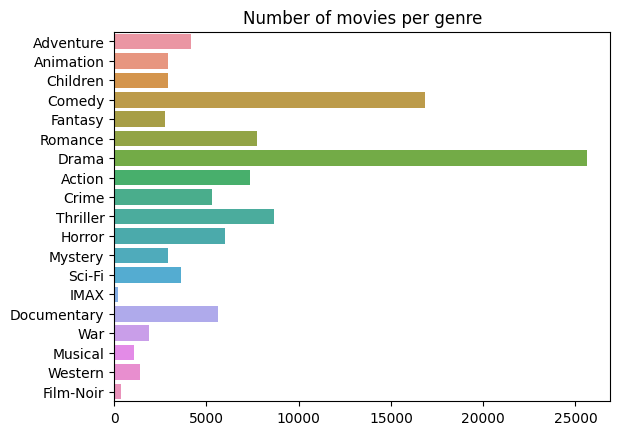
\includegraphics[width=1\textwidth]{img/genre_distribution.png}
  \caption{Répartition des genres dans la base de données}
\end{figure}

\newpage
\section{Question 2}
Le fichier \texttt{movies1.csv} a été créé en itérant sur les lignes du fichier
\texttt{movies.csv} et en ne gardant que les lignes dont le genre est défini. Pendant
cette itération, nous avons également stocké les moviesId des films avec un genre.
\vskip 0.25cm
Le fichier \texttt{ratings1.csv} a été créé en itérant sur les lignes du fichier
\texttt{ratings.csv} et en ne gardant que les lignes dont le movieId est présent
dans le fichier \texttt{movies1.csv}. Nous en avons profité pour arrondir les
notes de la manière préconisée par l'énoncé.
\vskip 0.25cm
Le fichier \texttt{movies1.csv} contient ainsi 57361 films sur les 62423 du
fichier \texttt{movies.csv}, et le fichier \texttt{ratings1.csv} contient
1569746 notes sur les 1571101 du fichier \texttt{ratings.csv}.

\section{Question 3}
La construction de la matrice binaire des genres des films est effectuée par
la fonction \texttt{movies\_stats} de notre module de gestion des données.
\vskip 0.25cm
Une matrice de taille $nb\_films \times nb\_genres$ remplie de 0 est créée grâce
à la fonction \texttt{zeros} de numpy. Ensuite, pour chaque film, on récupère
ses genres en itérant sur les lignes du fichier \texttt{movies1.csv} et on
remplit la matrice avec des 1 aux positions correspondantes aux genres du film.

\section{Question 4}
La construction de la matrice des profils des utilisateurs est effectuée par
la fonction \texttt{users\_stats} de notre module de gestion des données.
\vskip 0.25cm
Une matrice de taille $nb\_users \times nb\_genres$ remplie de 0 est créée puis
on itère sur les lignes du fichier \texttt{ratings1.csv} pour remplir la matrice.
Pour chaque ligne, on récupère la ligne correspondant au film dans la matrice
créée à la question précédente, on multiplie cette ligne par la note du film
et on ajoute le résultat à la ligne correspondant à l'utilisateur dans la matrice
des profils des utilisateurs.

\newpage
\section{Question 5}
\subsection{Normalisation des profils des utilisateurs}
Afin de rendre le clustering des centaines de fois plus rapide, nous avons
décidé de normaliser les profils des utilisateurs. Pour cela, nous avons
simplement divisé tous les coefficients de la matrice des profils des utilisateurs
par le maximum de la matrice afin que tous les coefficients soient compris
entre 0 et 1.

\subsection{Regroupement spectral des utilisateurs}
Le regroupement spectral des utilisateurs est effectué par la classe
\texttt{SpectralClustering} de \texttt{scikit-learn}. Nous avons utilisé le solver
\texttt{arpack} et la stratégie \texttt{kmeans} qui donnaient les meilleurs
résultats.
\vskip 0.25cm
En faisant varier nombre de clusters \texttt{k} de 2 à 5, nous avons pu determiner
que le nombre de clusters optimal était 2. Voici les résultats obtenus pour
les différentes valeurs de \texttt{k} en utilisant la métrique \texttt{silhouette\_score}
de \texttt{scikit-learn} :

\begin{figure}[ht]
  \centering
  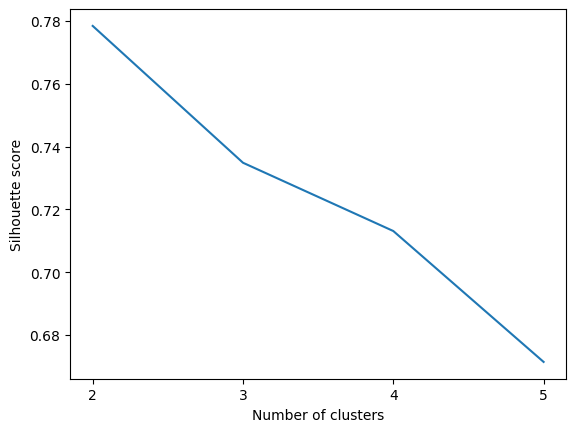
\includegraphics[width=1\textwidth]{img/silhouette_graph.png}
  \caption{\texttt{silhouette\_score} pour différentes valeurs de \texttt{k}}
\end{figure}

\subsection{Visualisation des clusters}
Nous avons utilisé plusieurs méthodes pour réduire la dimension des données
afin de pouvoir visualiser en 2 dimensions les clusters obtenus pour 
\texttt{$k \in \{2, 3, 4, 5\}$}.
\vskip 0.25cm
D'abord la classe \texttt{UMAP} de \texttt{umap-learn} dont voici les représentations :

\begin{figure}[ht]
  \centering
  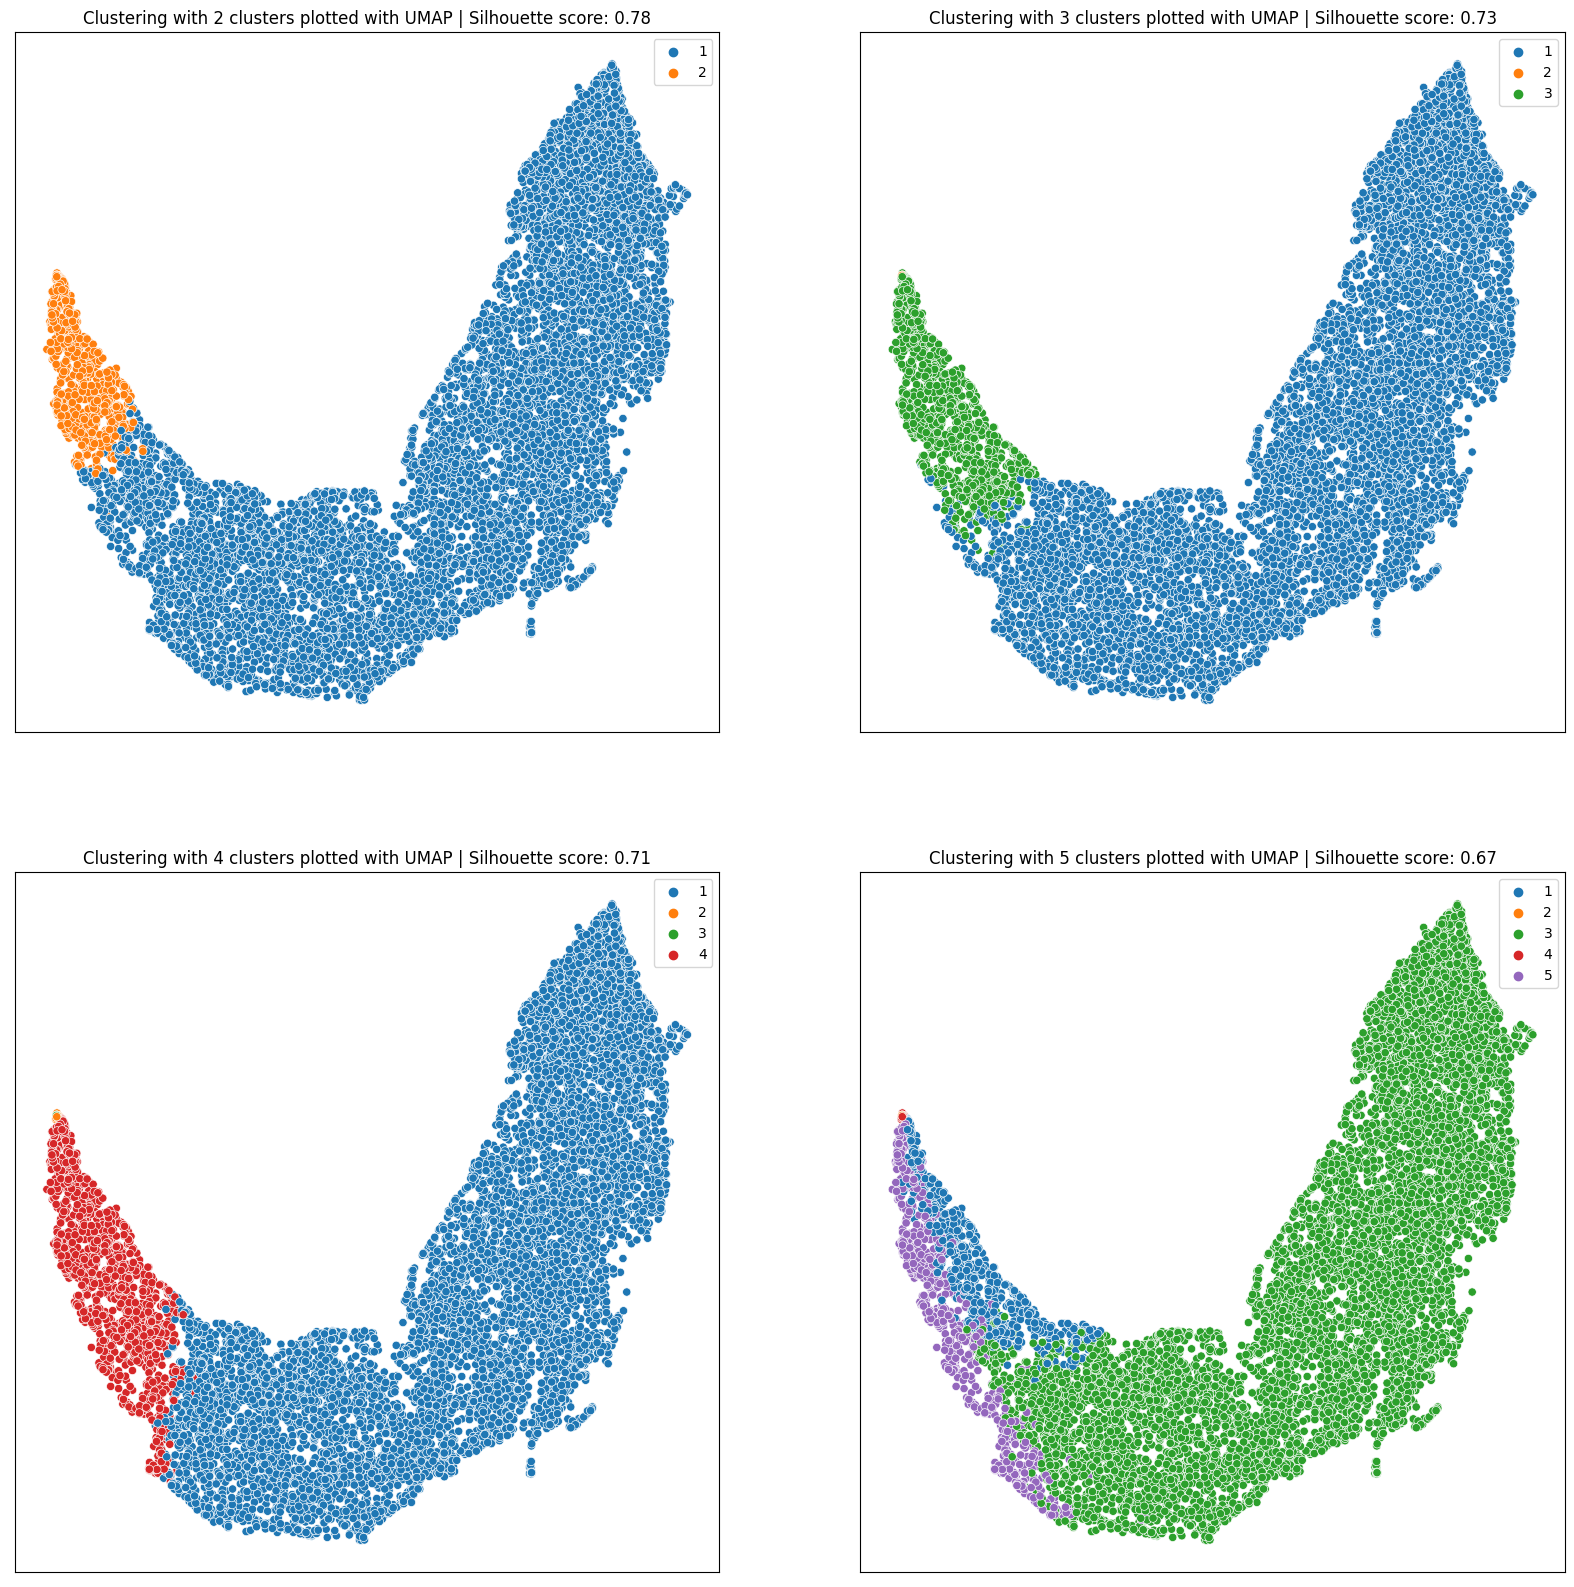
\includegraphics[width=1\textwidth]{img/clustering_umap.png}
  \caption{Visualisation des clusters pour différentes valeurs de \texttt{k} avec \texttt{UMAP}}
\end{figure}
\newpage

Ensuite la classe \texttt{PCA} de \texttt{scikit-learn} dont voici les représentations :

\begin{figure}[ht]
  \centering
  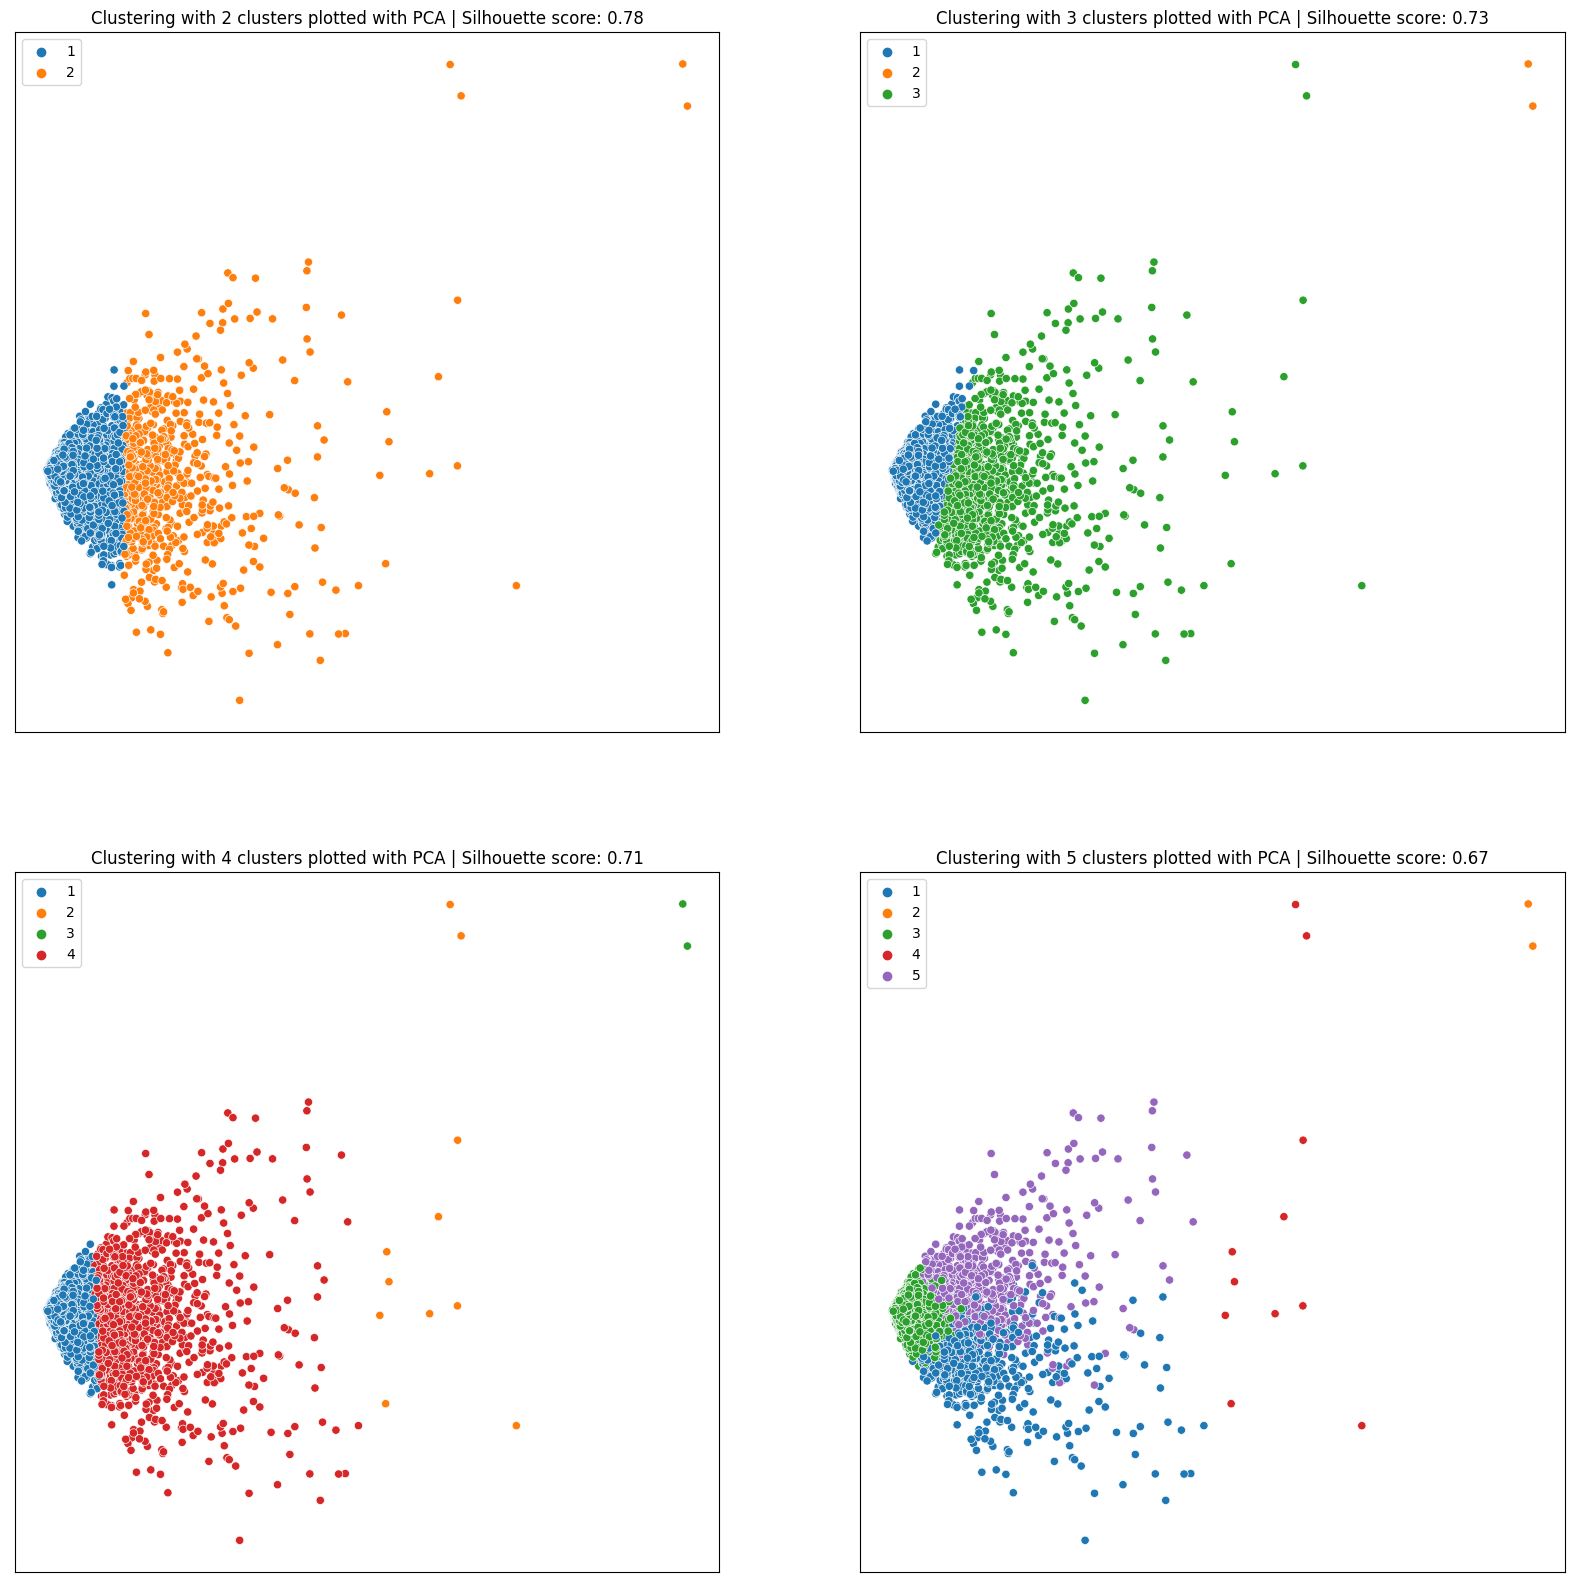
\includegraphics[width=1\textwidth]{img/clustering_PCA.png}
  \caption{Visualisation des clusters pour différentes valeurs de \texttt{k} avec \texttt{PCA}}
\end{figure}
\newpage

Enfin la classe \texttt{TSNE} de \texttt{scikit-learn} dont voici les représentations :

\begin{figure}[ht]
  \centering
  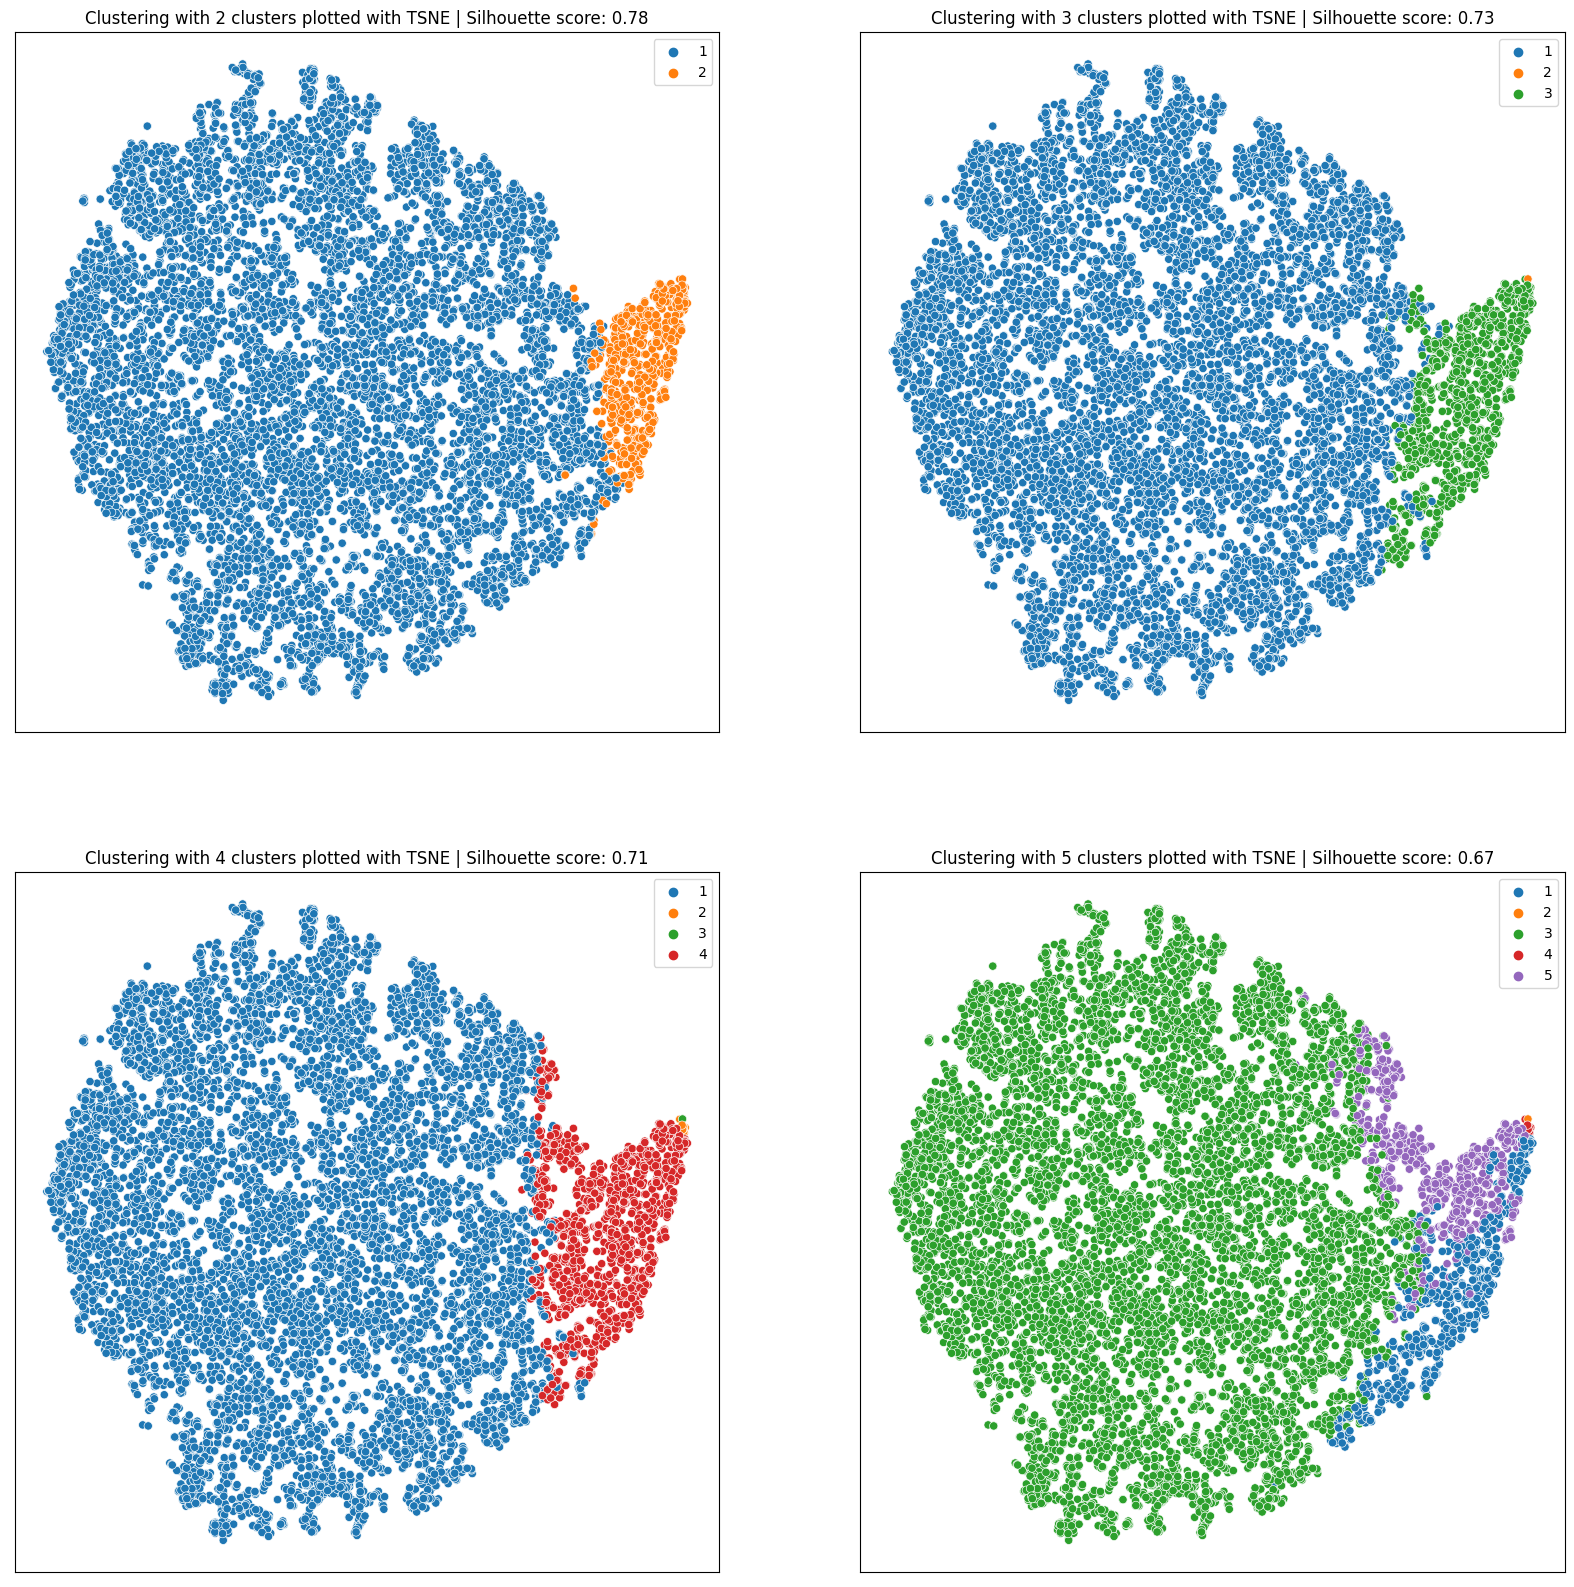
\includegraphics[width=1\textwidth]{img/clustering_TSNE.png}
  \caption{Visualisation des clusters pour différentes valeurs de \texttt{k} avec \texttt{TSNE}}
\end{figure}
\newpage

Il semble que les clusters obtenus soient très déséquilibrés, nous avons donc
affiché la répartition des utilisateurs dans les clusters afin de confirmer
cette hypothèse :

\begin{figure}[ht]
  \centering
  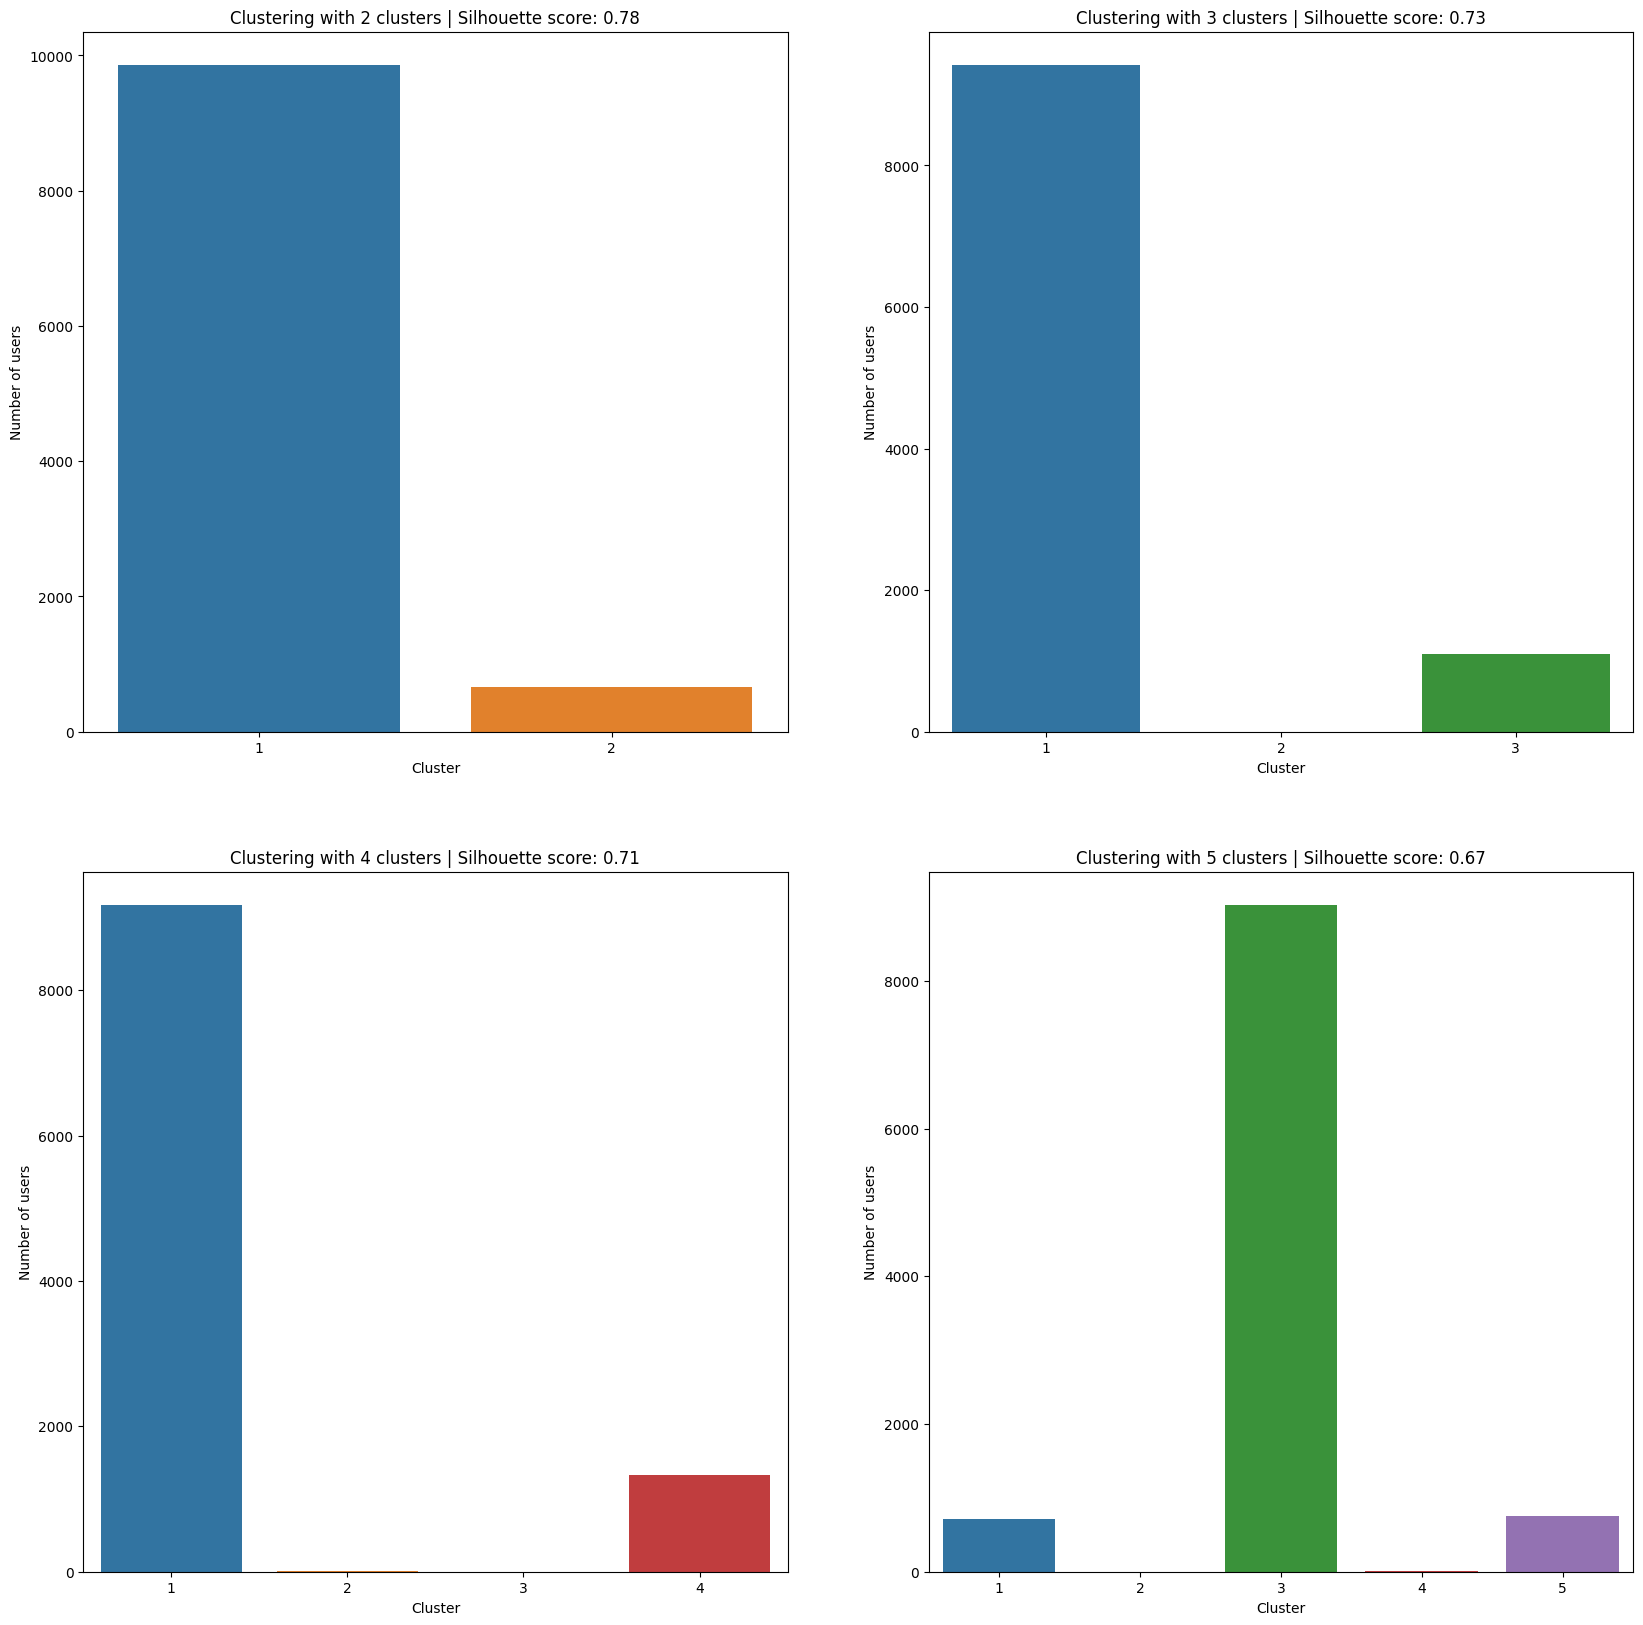
\includegraphics[width=1\textwidth]{img/clusters_distribution.png}
  \caption{Répartition des utilisateurs dans les clusters pour différentes valeurs de \texttt{k}}
\end{figure}

\newpage
\section{Question 6}

\subsection{Préparation des ensembles}
Nous avons utilisé la fonction \texttt{StratifiedShuffleSplit} de \texttt{scikit-learn}
pour séparer les données en 3 ensembles : un ensemble d'entraînement, un ensemble
de validation et un ensemble de test avec des proportions respectives de 60\%,
20\% et 20\%.
\vskip 0.25cm
Cette fonction nous permet de conserver la répartition des notes dans les
différents ensembles.
\vskip 0.25cm
On obtient ainsi 3 fichiers \texttt{ratings\_train.csv}, \texttt{ratings\_evaluation.csv}
et \texttt{ratings\_test.csv} contenant respectivement 941847, 313950 et 313950 notes.

\subsection{Prétraitement des données}
Afin de pouvoir entraîner l'arbre de décision, il faut d'abord trouver pour chacune
des notes laissées par les utilisateurs, les notes des 5 utilisateurs les plus
proches ayant noté le même film.
\vskip 0.25cm
Nous avons utilisé l'attribut \texttt{affinity\_matrix\_} de la classe
\texttt{SpectralClustering} pour obtenir la matrice
des similarités entre les utilisateurs qui découle de leur regroupement spectral.
Cette matrice de taille $nb\_users \times nb\_users$ contient au coefficient
$(i, j)$ la similarité entre les utilisateurs $i$ et $j$ vis-à-vis de leur profil.
\vskip 0.25cm
Le prétraitement des données est effectué par la fonction \texttt{five\_closest\_users}
de notre module de prétraitement des données. Pour chaque note, trie les utilisateurs
selon leur similarité avec l'utilisateur qui a laissé la note et ne garde que les
5 utilisateurs les plus proches ayant noté le même film. Si moins de 5 autres utilisateurs
ont noté le même film, la note est ignorée.
\vskip 0.25cm
On obtient finalement un dictionnaire avec des entrées de la forme 
\texttt{(userId, movieId, rating) : [r1, r2, r3, r4, r5]} où \texttt{r1, r2, r3, r4, r5}
sont les notes des 5 utilisateurs les plus proches ayant noté le même film.

\subsection{Recherche des hyperparamètres optimaux}
Afin de trouver les hyperparamètres optimaux pour l'arbre de décision, nous avons
utilisé la classe \texttt{GridSearchCV} de \texttt{scikit-learn} qui permet
de faire une recherche exhaustive à travers une grille de paramètres qui
contient pour chaque hyperparamètre une liste de valeurs à tester.
\vskip 0.25cm
\noindent Nous avons testé les valeurs suivantes des hyperparamètres suivants :

\begin{itemize}
  \item \texttt{criterion} : \texttt{['gini', 'entropy']}
  \item \texttt{splitter} : \texttt{['best', 'random']}
  \item \texttt{max\_depth} : \texttt{[None, 5, 10, 50, 100, 200, 500]}
  \item \texttt{min\_samples\_split} : \texttt{[2, 5, 10, 20, 50, 100]}
  \item \texttt{min\_samples\_leaf} : \texttt{[1, 2, 5, 10, 20, 50, 100]}
  \item \texttt{max\_features} : \texttt{['sqrt', 'log2']}
\end{itemize}

\noindent Voici les paramètres optimaux obtenus :

\begin{itemize}
  \item \texttt{criterion} : \texttt{'gini'}
  \item \texttt{splitter} : \texttt{'best'}
  \item \texttt{max\_depth} : \texttt{50}
  \item \texttt{min\_samples\_split} : \texttt{20}
  \item \texttt{min\_samples\_leaf} : \texttt{100}
  \item \texttt{max\_features} : \texttt{'sqrt'}
\end{itemize}

Nous avons remarqué qu'en réalité, la plupart des combinaisons d'hyperparamètres
donnent des résultats similaires, et que les hyperparamètres optimaux donnent
des performances à peine meilleures que les paramètres par défaut.

\subsection{Entraînement et prédictions de l'arbre de décision}
L'arbre de décision est entraîné par la classe \texttt{DecisionTreeClassifier}
de \texttt{scikit-learn} avec les hyperparamètres optimaux trouvés précédemment 
sur l'ensemble d'entraînement et évalué sur l'ensemble d'évaluation.
\vskip 0.25cm
Les entrées sont les valeurs du dictionnaire créé en 6.3 et les notes prédites
sont comparées avec la note qui apparaît dans la clé du dictionnaire et qui est
la note réelle laissée par l'utilisateur.
\vskip 0.25cm
La métrique utilisée pour évaluer l'arbre de décision est le F1-score
qui est la moyenne harmonique de la précision et du rappel. Nous avons donc 
utilisé la fonction \texttt{f1\_score} de \texttt{scikit-learn} pour calculer
le \texttt{f1-score} des prédictions de l'arbre de décision sur l'ensemble
de test.

\subsection{Résultats}
Le F1-score obtenu sur l'ensemble de test pour les hyperparamètres optimaux
trouvés précédemment est de $0.32$.
\vskip 0.25cm
Trouvant ce score assez faible, nous avons essayé de comprendre pourquoi
l'arbre de décision ne fonctionnait pas très bien. Nous avons alors décidé
de calculer le F1-score en considérant comme un Vrai Positif une prédiction
de l'arbre de décision qui était à 1 point ou moins de la note réelle.
\vskip 0.25cm
Nous avons alors obtenu un F1-score de $0.82$ ce qui est beaucoup plus
satisfaisant. Cela signifie que même si l'arbre de décision ne prédit pas
exactement la note réelle, il prédit une note très proche de la note réelle.
\vskip 0.25cm
Finalement, malgré un F1-score assez faible, notre système de recommandation
basé sur un arbre de décision semble fonctionner assez bien.

\end{document}
